\section{Manual de usuario}
Dado que el paquete desarrollado dispone de toda la documentaci\'on necesaria, accesible a trav\'es de Rstudio, dicha documentaci\'on se constituye como el manual de usuario del paquete. 

Esta documentaci\'on ha sido desarrollada tal y como se describe en la secci\'on 2, por lo que tambi\'en est\'an contempladas las dependencias del paquete y, por tanto, solo con instalarlo desde Rstudio ya es posible hacer uso del mismo. Por lo que los requisitos para la instalaci\'on y uso del paquete, no son m\'as que tener instalada una versi\'on actualizada de R y de Rstudio.

A continuaci\'on, se pueden ver ejemplos de acceso a la documentaci\'on del paquete desde Rstudio.
\begin{figure}[H]
    \centering
    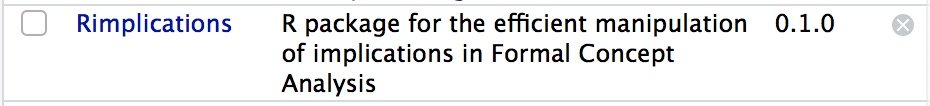
\includegraphics[scale=0.75]{docs1}
    \caption{Ejemplo Documentaci\'on 1}
    \label{fig:docs1}
\end{figure}

\begin{figure}[H]
    \centering
    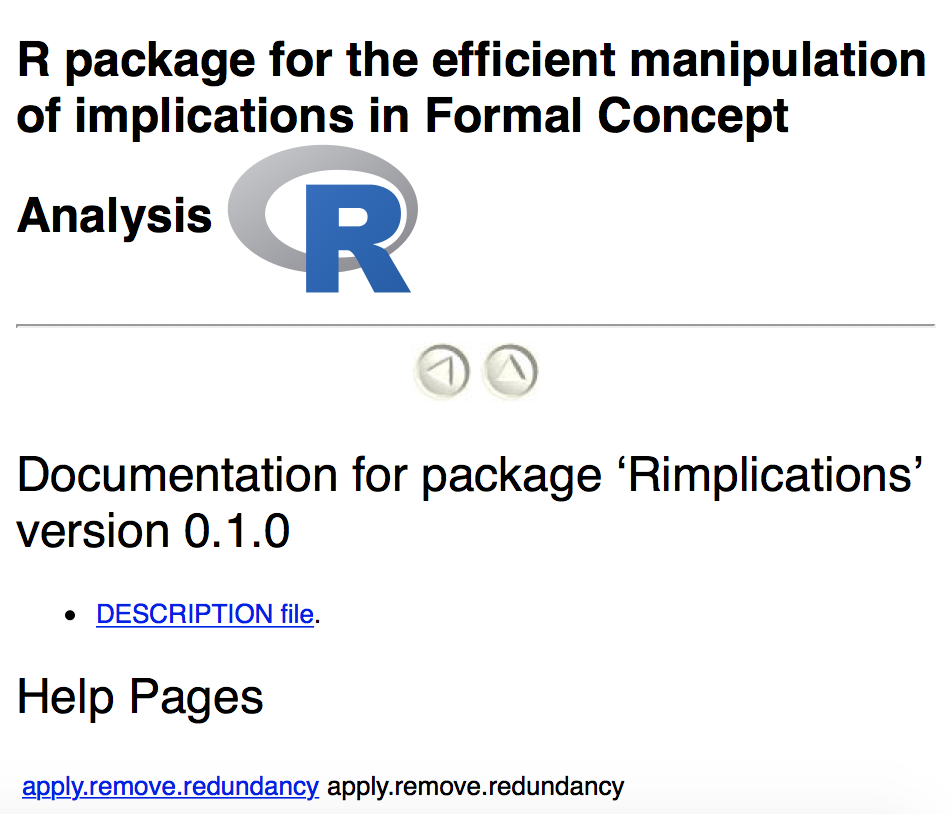
\includegraphics[scale=0.6]{docs2}
    \caption{Ejemplo Documentaci\'on 2}
    \label{fig:docs2}
\end{figure}

Aqu\'i se ve la documentaci\'on del algoritmo para la eliminaci\'on de redundancia:
\begin{figure}[H]
    \centering
    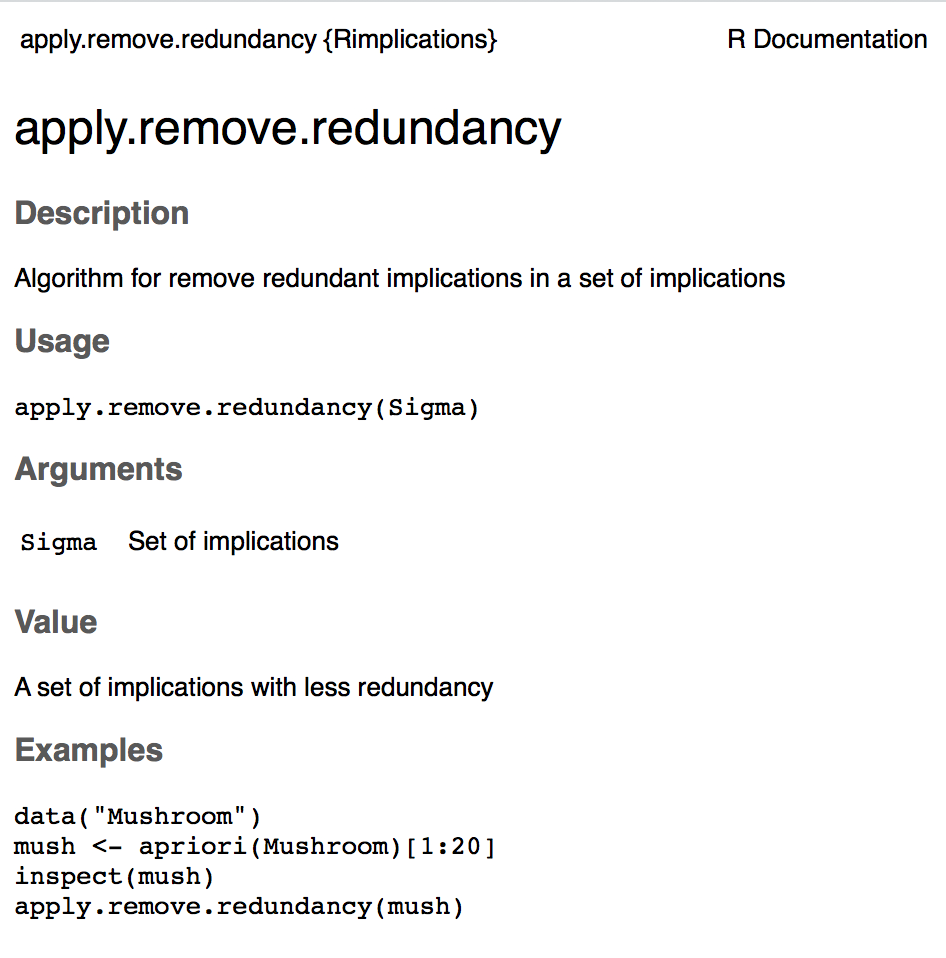
\includegraphics[scale=0.75]{docs3}
    \caption{Ejemplo Documentaci\'on 3}
    \label{fig:docs3}
\end{figure}
\newpage